\chapter{Zdroje dát pre analýzu}
\label{data-sources-available-for-research}

Pre účely analýzy využívania technológie NEL je nutné získať pohľad do diania vo verejnom internete.
Cieľom je pozerať sa na reálne komunikácie, ktoré buď už prebehli, alebo skúmať ako určité webové služby aktuálne dostupné na internete
odpovedajú na HTTP(S) požiadavky. V tejto kapitole sú detailne popísané dostupné zdroje dát 
a ktoré z nich sú reálne aj použité v praktickej časti tejto práce. % TODO -- kapitole \ref{analysis-and-its-results}.

\section{Potrebné dáta}

To čo je potrebné zaobstarať pre analýzu v tejto práci sú záznamy konkrétnych služieb, z ktorých možno čerpať aktuálny alebo historický stav. Čo sa týka štruktúry, v ideálnom prípade by išlo o presný výpis všetkých \textbf{webových domén dostupných verejne na internete}, ktoré možno skúmať. 
Zoznam spĺňajúci takýto popis je potrebné zaobstarať práve preto, aby sme jednak vedeli, ktoré domény je vôbec možné analyzovať a ďalej preto, aby sme vo výsledkoch práce vedeli s touto informáciou pracovať a spájať relevantné vzťahy. Napríklad medzi doménou a jej vlastníkom. 
Práve touto spojitosťou sa môžeme dostať napríklad k prehľadu o tom, kto vlastní najvyšší počet domén využívajúcich NEL. 
Takýchto zoznamov existuje hneď niekoľko a sú spomenuté v ďalšej sekcií, sekcií číslo \ref{tranco}, kde sú do detailu popísané aj ich dôležité vlastnosti. 
Taktiež v nej popisujem ten najvhodnejší z uvedených zoznamov.

Následne, keď by už je známe, ktoré domény je možné podrobiť analýze, je ďalej nutné k nim prideliť aj dáta týkajúce sa ich reálneho sieťového prenosu.
Keďže sa v práci zameriavam na technológiu NEL, pod sieťovým prenosom je myslený menovite protokol \textbf{HTTPS}, v ktorom majú byť preverené prítomnosti hlavičiek NEL. 
Existujú dva pohľady na tento prenos:
\begin{enumerate}
    \item Aktuálne dáta:
    
    Z hľadiska prítomnosti, a teda aktuálneho stavu webových technológií je vhodné použiť napríklad techniku takzvanú \textbf{Web Crawling}.
    Na účel Web Crawlingu je možné použiť už existujúce technológie ako \textbf{Selenium}. 
    Selenium opisuje sekcia \ref{selenium}.

    \pagebreak
    
    \item Historické dáta:

    Aby bol nadobudnutý prehľad vývoja nasadenia NEL v čase, je nevyhnutné nahliadnuť taktiež do histórie prevádzky vo webe. 
    V tomto bode je zasa nutné hľadať už spracované a uložené dáta získané či už Web Crawlingom, alebo inými spôsobmi. 
    Vyhovujúcim zdrojom takýchto historických dát je napríklad projekt \textbf{HTTP Archive}, ktorému sa práca venuje primárne, a to v sekcií \ref{httparchive}.
    Ide o službu, ktorá zaznamenáva vývoj webu od roku 2010 a teda jej vhodnosť sa potvrdzuje tým, že samotná špecifikácia NEL v tejto práci bola publikovaná až v roku 2018.
\end{enumerate}

% V oblasti zdrojov historických dát sa nachádzajú aj určité alternatívy, ktoré je možné využiť komplementárne k spomenutému primárnemu zdroju.
% Im je tu venovaná iba okrajová pozornosť, no každá z nich ale za zmienku nepopierateľne stojí, a preto sú popísané v kapitole \ref{httparchive-alternatives}.


\section{Zoznamy populárnych domén}
\label{tranco}

Ako už bolo spomenuté, vzniká potreba zaobstarania si zoznamu domén, s ktorými možno pracovať. Čo sa vlastností takýchto domén týka,
musia vystavovať verejnému internetu službu, ktorá je dosiahnuteľná, komunikuje protokolom HTTPS, a ideálne je aj často navštevovaná,
a tým pádom relevantná pre túto prácu. 
Najviac prichádza do úvahy zamerať sa na získanie zoznamu \textbf{webových domén}, zoradeného podľa
ich návštevnosti, ktorý bude zároveň nadobúdať dostatočne veľký rozsah pre účely prieskumu. 

Zaobstarávaniu zoznamov domén, ktoré majú spĺňať konkrétne predurčené kritéria sa venuje rad iných existujúcich služieb 
\cite{hacker-target-website-lists-overview, tranco}. Táto práca namiesto implementovania vlastného riešenia využíva jedno z nich -- TRANCO.

TRANCO je rebríček webových domén zoradených podľa hodnotenia ich návštevnosti, ktorý je odolný proti externej manipulácií a vhodný na účely výskumu \cite{tranco-homepage}. 
Vznikol na základe častej potreby pre skúmanie práve takýchto domén či už pre jednoduchú referenciu, alebo ako podklad pre ďalší prieskum.
TRANCO nie je prvým takýmto rebríčkom, ale je prvým, ktorý sa zaoberá nedostatkami iných existujúcich rebríčkov.
Tieto ostatné rebríčky využíva ako zdroje dát pre tvorbu svojho rebríčka (viď sekciu \ref{tranco-source-rankings}).
Nový rebríček TRANCO tvorí \textbf{spájaním ostatných zdrojových rebríčkov} do nového, 
ktorý je stabilnejší, reprezentuje domény v globálnej škále a dokonca do určitej miery odstraňuje domény, na ktorých je môže byť zverejnený nežiadúci (nebezpečný) obsah\cite{tranco}. 

Obsahuje primárne registrovateľné domény, čo sú domény, ktoré si môže priamo zakúpiť či už jednotlivec alebo organizácia. 
Príkladom môžu byť domény registrované pod TLD \code{.com}, ale aj domény registrované pod eTLD zo zoznamu verejných suffixov ako \mbox{\code{*.co.uk} \cite{tranco}}. 
Okrem registrovateľných domén je možné vygenerovať rebríček aj s ich subdoménami (viď sekciu \ref{tranco-generation}).
Vygenerované rebríčky možno použiť napríklad na analyzovanie využitia konkrétnych webových technológií na týchto doménach -- od použitej metódy komprimácie jej obsahu po rámce, pomocou ktorých bola webová služba na nich vyvinutá.

TRANCO som si pre svoju prácu vybral hlavne preto, že sprístupňuje dáta jednotlivých rebríčkov, ktoré vnútorne používa. 
Niektoré z tých rebríčkov už nie sú dostupné samostatne, a preto je nutné použiť TRANCO, ktorý obsahuje aj historické dáta z nich. 
Je teda vhodné použiť toto riešenie použiť pre vytvorenie vlastnej kombinácie zdrojových rebríčkov vhodnej pre špecifickú analýzu domén výsledného rebríčka TRANCO (viď možnosti konfigurovania v sekcii \ref{tranco-config}), alebo pre či už replikovanie a overenie predošlých prác, ktoré používali zastarané rebríčky (viď kapitolu \ref{related-work}).

\pagebreak


\subsection{Zdrojové rebríčky domén}
\label{tranco-source-rankings}

Ako už bolo zmienené vyššie, stratégia získavania domén, ktoré následne TRANCO podrobí hodnoteniu spočíva vo vyberaní týchto domén z už existujúcich rebríčkov s hotovým hodnotením. 
Zdrojom dát pre hodnotenie domén TRANCO je teda množina niekoľkých podobných rebríčkov, ktoré sami na ich úrovni používajú rôzne stratégie pre obstarávanie domén a ich zoraďovanie 
podľa hodnotenia návštevnosti \cite{tranco-methodology}. 
V tejto kapitole sú popísané rebríčky, z ktorých možno dáta kombinovať 
a na základe ktorých je možné nový alebo vlastný rebríček vygenerovať.

\subsubsection{Alexa}

Alexa, dcérska spoločnosť Amazon.com, publikovala na svojich stránkach od decembra 2008 až po začiatok augusta 2023 rebríček \textbf{Alexa Top Sites}, v ktorom zoraďovala 1 milión 
najnavštevovanejších domén web serverov \cite{tranco-methodology}.
Zdrojom dát pre jeho tvorbu bolo rozšírenie pre webové prehliadače, ktoré si používatelia mohli stiahnuť a po jeho inštalácií na vybranom prehliadači začalo zbierať a odosielať
dáta o prehliadaní internetu do Alexy. 
Pre účely vytvorenia hodnotenia domén sa teda využíva sieťová prevádzka priamo vedená cez protokol HTTP(S). 
Rebríček Alexa sa v tomto skúmaní HTTP(S) prevádzky zaoberá registrovateľnými doménami. 

Počet používateľov s nainštalovaným rozšírením bol však obmedzený 
a to mohlo spôsovovať značné skreslenie celkových výsledkov kvôli malému zastúpeniu vzoriek prehliadania z celkovej sady -- všetkých používateľov internetu. 
Avšak, existujú zmienky, kde sa cituje pôvodná oficiálna stránka tohto rebríčka, kde autori tvrdili, že počet týchto používateľov sa pohyboval v ráde niekoľkých miliónov \cite{tranco}.
Svoje hodnotenie Alexa zakladala na dvoch základných metrikách: \cite{kinsta-alexa-rank-article, tranco}
\begin{itemize}
    \item Počet návštevníkov stránky (na web serveri s danou doménou) za daný deň, pričom viac návštev od jedného používateľa sa počíta ako jediná návšteva
    \item Spriemerovaný počet otvorení hocijakej podstránky (URL v rámci sledovanej domény)
\end{itemize}

Zo spomenutých metrík má vyššiu váhu pri rozhodovaní o popularite práve počet návštevníkov stránky za daný deň, čo môžeme podľa jej popisu nazvať aj počet unikátnych návštev za deň \cite{tranco}.
Obe metriky sa pre špecifický deň následne spriemerovali so všetkými hodnotami za posledné tri mesiace, aby rebríček nadobudol určitú mieru stability. 
Tým pádom každodenný rebríček nepripúšťa do úvahy trendy v prehliadaní, ktoré po vzniknutí hneď aj zanikajú (krátkodobé extrémy). 
Vo výsledku sa tým predchádza nepresnému celkovému hodnoteniu popularity v prípadoch, 
kedy by neobvyklý jednorazový nárast v popularite doposiaľ neznámej domény mal predbehnúť zaradenie inej, dlhodobo populárnej a vysoko zaradenej domény v rebríčku. 

Koncom roka 2016 bol tento bezplatne poskytovaný rebríček na nejakú dobu odstavený z prevádzky pre verejnosť na hlavných stránkach Alexy a znova bol sprístupnený pod záštitou Amazon Web Services ako platená služba \textbf{Alexa Top Sites}. 
Neskôr, začiatkom roka 2018 sa zhoršila jeho celková stabilita z toho dôvodu, že jeho algoritmus vyhodnocovania zaradenia domén prestal brať ohľad na priemerovanie dát za predošlé mesiace.
Od vtedy, konkrétne od 30. januára 2018, bol zhotovovaný striktne iba za každý konkrétny deň \cite{tranco} až dokým táto služba nebola nadobro prerušená 1. augusta 2023, čo z nej teraz robí \mbox{\textbf{zastaraný rebríček} \cite{tranco-methodology}}.

\subsubsection{Majestic Million}

Majestic Million je služba, ktorá rovnako ako Alexa poskytuje rebríček webových domén zoradených podľa množstva odkazov na ne ukazujúcich \cite{majestic-million-homepage, majestic-million-ranking}.
V jednoduchosti to znamená, že čím viac odkazov na danú doménu sa na webe nájde, tým vyššie bude v tomto rebríčku zaradená. 
Ako individuálne technologické riešenie bol Majestic Million uverejnený na webových stránkach autora 1. októbra 2012 \cite{majestic-million-publication}.
Autorom je spoločnosť Majestic, ktorá sa zaoberá SEO (Search Engine Optimization) a skúmaním práve takýchto prepojení medzi doménami.

Majestic na dennej báze prehľadáva globálne zhruba 450 miliárd URL v rámci verejného internetu aby svoj rebríček zostavil. 
Hodnotenie je založené na počte hyperlinkových odkazov smerujúcich na jednotlivé hodnotené domény minimálne jedenkrát.
Okrem každodenného vyhodnocovania aktuálneho zaradenia domén sa taktiež berie ohľad aj na priemer ich hodnotenia za posledných 120 dní \cite{tranco-methodology}.
Tiež je vhodné spomenúť, že autori na svojom webe označujú vysoké zaradenie domény v tomto rebríčku za znak dôveryhodnosti \cite{majestic-million-homepage}.

V rámci celkového výstupného rebríčka Majestic Million sa berú do úvahy domény, \textbf{ale aj ich subdomény}, takže sa môže stať, že napríklad doména \code{google.com} 
sa v ňom bude vyskytovať viackrát v podobe svojich subdomén (\code{play.google.com}, \code{maps.google.com}, \code{mail.google.com} a iné) \cite{majestic-million-sub-domain-filtered}.

Na oficiálnom webe Majestic sú taktiež dostupné doplnkové služby, ktoré svojim používateľom poskytujú naväzujúce užitočné informácie o týchto doménach. 
Jednou z nich je napríklad možnosť bližšie porovnať až do 10 domén, kde vstupom sú ich mená a výstupom je prehľadná tabuľka (takzvaná Buzz Table) zobrazujúca ich zaradenie a iné detaily, medzi ktoré patrí aj počet domén
referujúcich na tie vstupné a aj celkový počet ich externých odkazov \cite{majestic-million-homepage}.
Existujú rôzne ďalšie služby, ktoré Majestic ponúka, no až na samotný rebríček a spomenutý Buzz Table sú tie ostatné spoplatnené, kde najlacnejšia možnosť platobného plánu v čase písania práce začína na \$46.99 mesačne \cite{majestic-million-pricing}.

\subsubsection{Cisco Umbrella}
% TODO nemusi byt https obsah

Rebríček Cisco Umbrella obsahuje zoradenie najviac navštevovaných stránok podľa prekladu ich doménových mien na IP adresy na DNS serveroch patriacich spoločnosti Cisco.
Tieto DNS servery sú súčasťou globálnej siete Cisco Umbrella, kde sa cez deň nahromadí viac ako 100 miliárd požiadaviek na rezolúciu od 65 miliónov aktívnych užívateľov z viac ako 165 krajín.
Narozdiel od rebríčka Alexa používa Cisco Ubrella namiesto HTTP požiadaviek jedinečné IP adresy klientov na identifikáciu návštev na kontrolované domény.
Rebríček je generovaný každodenne a obsahuje 1 milión záznamov s top-level doménami (TLD) \textbf{a ich subdoménami}, ktoré Alexa nezahŕňa \cite{cisco-umbrella}.

Je ale nutné poznamenať, že vzhľadom na to, že sa ako zdroj využívajú záznamy DNS, do finálneho rebríčka sa dostávajú aj nedosiahnuteľné domény.
Medzi také patria domény, ktoré sú interné pre špecifickú organizáciu používajúcu službu Cisco Umbrella, a teda sú neprístupné pre bežného návštevníka.
Ďalej sa môžu na nižších miestach vyskytnúť neexistujúce domény, ktoré boli zaradené do rebríčka len vďaka častým DNS vyhľadávaním s chybou v názve danej domény (napríklad \code{google.comm}) \cite{tranco-methodology}.

\pagebreak

\subsubsection{Quantcast}

Spoločnosť Quancast zverejňovala do 1. apríla 2020 rebríček najnavštevovanejších stránok v Spojených Štátoch Amerických (US). Jeho veľkosť sa denne menila, no bežne v ňom bývalo
okolo 520,000 registrovateľných domén a subdomén. Quantcast zaraďoval tieto domény do svojho rebríčka podľa počtu ľudí, ktorí ich navštívili vždy za predošlý mesiac.
Návštevnosť sa merala pomocou sledovacieho skriptu umiestneného na samotných doménach alebo podľa dát získaných od poskytovateľov internetu (ISP) \cite{tranco-methodology}.

Limitácia tohto rebríčka spočíva okrem toho, že už je zastaraný a neautualizovaný, a taktiež v tom, že berie ohľad v drvivej väčšine prípadov na stránky v US.
Jedinou výnimkou boli domény mimo US, ktoré využívali spomínaný sledovací skript. 

\subsubsection{Chrome User Experience Report}

% \todo{}
Táto sekcia ešte nie je napísaná.

\subsubsection{Cloudflare Radar}

Po ohlásení ukončenia podpory pre rebríček Alexa sa spoločnosť Cloudflare rozhodla poskytnúť vhodnú alternatívu.
Od 26. septembra 2022 zverejňujú rebríček Radar obsahujúci registrovateľné domény, ktorý je aktualizovaný podľa svojej veľkosti na dennej alebo týždennej báze \cite{tranco-methodology}.

Dáta o návštevnosti domén sú získavané zo sieťovej premávky na Cloudflare DNS serveri s IP adresou \code{1.1.1.1}.
Tento server je verejný Cloudflare DNS server, ktorý sprostredkuje rýchly a súkromný spôsob prehliadania internetu.
Je považovaný za najrýchlejší DNS server a zároveň nepredáva dáta o svojich používateľoch. % TODO \ref{cloudflare}.

Umiestnenia domén v rebríčku sú vypočítané na základe metriky popularity, ktorá predstavuje podľa popisu od Cloudflare "\textit{odhadovanú relatívnu veľkosť populácie užívateľov, ktorí navštívili doménu za určitú dobu}".
Táto metrika sa vypočítava použitím modelu strojového učenia na agregované dáta zo spomínaného DNS servera. 

Špecifikom tohto rebríčka je rozdelenie výsledných domén do takzvaných \textbf{buckets} (bucket, anglicky vedro) o postupne zvyšujúcich sa veľkostiach.
Veľkosť prvého, jediného bucketu, ktorý je aktualizovaný každý deň je 100 domén. Tieto domény sú medzi sebou vzájomne zoradené.
Nasledujúce buckets majú jednotlivé veľkosti 200, 500, 1,000, 2,000, 5,000, 10,000, 20,000, 50,000, 100,000, 200,000, 500,000 a 1,000,000 domén.
Domény v týchto početnejších zoznamoch už nie sú zoradené vzájomne medzi sebou.
Ich význam spočíva v tom, že každý bucket predstavuje relatívnu vzdialenosť začlenených domén od tej najpopulárnejšej \cite{cloudflare-radar}.



\subsection{Generovanie rebríčka TRANCO}
\label{tranco-generation}

V jeho štandardnej forme, rebríček TRANCO sa generuje každý deň v dvoch verziách:
\begin{itemize}
    \item TRANCO rebríček domén
    \item TRANCO rebríček domén a subdomén
\end{itemize}

\pagebreak

V tomto každodenne generovanom rebríčku sú prednastavené ako zdroje dát (použité existujúce rebríčky), tak aj dátumový rozsah, za ktorý sa zo zdrojových rebríčkov má čerpať.
Štandardne sa teda vytvára výsledok z rebríčkov Alexa, Umbrella, Majestic a Quantcast, ktoré bližšie predstavuje nasledujúca časť tejto sekcie. 
Dátumový rozsah je nastavený na posledných 30 dní \cite{tranco-github}, pričom TRANCO použije ako kompletný zdroj dát všetky spomenuté rebríčky vygenerované za túto dobu. 

V novom TRANCO rebríčku sa zo zdrojových rebríčkov spriemeruje pre každú doménu jej zaradenie aplikovaním jednej z dostupných kombinačných metód pre upravenie finálneho hodnotenia domén.
Pre štandardný rebríček je využitá kombinačná metóda takzvanej harmonickej progresie, nazývaná \textbf{Dowdall rule}. 
Dowdall rule hodnotí v zozname obsahujúcom N domén prvú hodnotou 1 a všetky ostatné postupne \(1/2\), \(1/3\) až \(1/(N-1)\) a zakončí hodnotením poslednej -- \(1/N\) \cite{tranco, tranco-homepage}.
Názorná ukážku aplikovania Dowdall rule na rebríčky ukazuje obrázok \ref{img:dowdall-rule}.

\begin{figure}[htb]
\begin{center}
 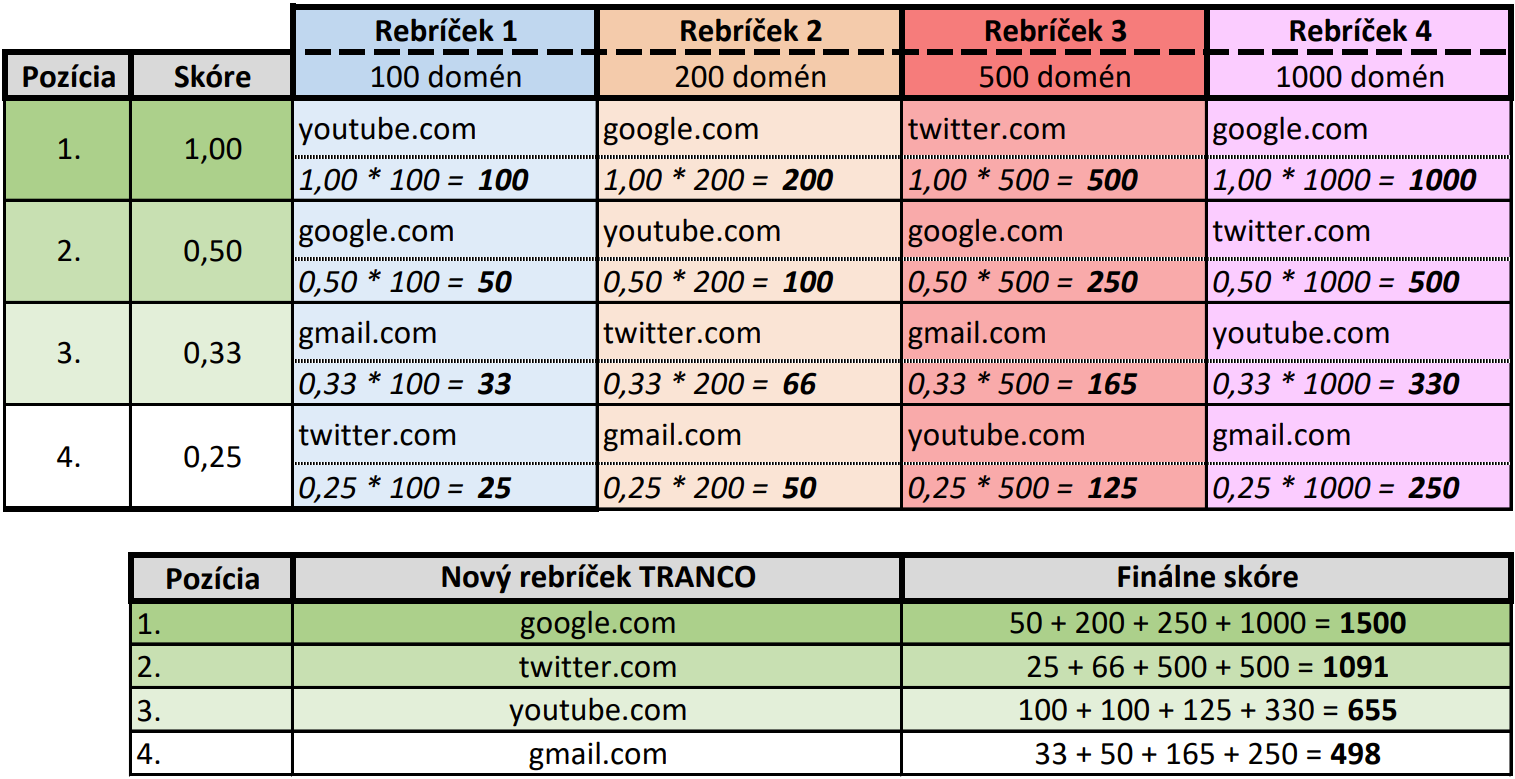
\includegraphics[scale=0.375]{obrazky-figures/dowdall_rule.png}
 \caption{\centering Príklad uplatnenia Dowdall rule na spriemerovanie štyroch vstupných rebríčkov do výsledného rebríčka TRANCO. Generujem nový rebríček o veľkosti štyroch domén, takže beriem do úvahy prvé štyri domény z každého vstupného rebríčka. Skóre sa vypočíta podľa umiestnenia a podľa celkového počtu domén radených v danom zdrojovom rebríčku. Rebríček 4 (úplne napravo) s najvyšším počtom hodnotených domén výsledok ovplyvnil najviac.}
 \label{img:dowdall-rule}
\end{center}
\end{figure}



Po dokončení priemerovania a zaraďovania sa spolu s výsledným rebríčkom vytvorí na oficiálnom webe TRANCO aj jedinečná stránka obsahujúca odkaz na jeho stiahnutie a tiež citácia, 
ktorou je možné jedinečne odkazovať na tento nový rebríček v prácach, ktoré ho môžu použiť na svoje účely.

Zároveň, okrem generovania nových TRANCO rebríčkov sú na oficiálnej stránke dostupné aj historicky vygenerované, spomenuté \textbf{štandardné}, teda bežné, každodenné rebríčky \cite{tranco-homepage}.
Príklad obsahu vygenerovaného rebríčka znázorňuje výpis \ref{listing:tranco-obsah}.



\pagebreak

\begin{center}
\centering
\begin{lstlisting}[caption={\centering Ukážka vygenerovaného denného rebríčku z 12. januára 2024, orezaného na prvých 10 domén. Rebríček je možné stiahnuť vo formáte \code{zip} archívu, ktorý obsahuje práve jeden súbor nazvaný \textbf{top-1m.csv}. Obsahom je na každom riadku pozícia domény a jej čiarkou oddelené meno.},
label=listing:tranco-obsah, 
language=json, 
frame=lb,
xleftmargin=.3875\textwidth, 
xrightmargin=.3875\textwidth]
1,google.com
2,amazonaws.com
3,facebook.com
4,microsoft.com
5,a-msedge.net
6,googleapis.com
7,apple.com
8,youtube.com
9,akamaiedge.net
10,akamai.net

\end{lstlisting}
\end{center}




\subsubsection{Možnosti konfigurácie vlastného rebríčka TRANCO}
\label{tranco-config}

Na oficiálnej stránke TRANCO je taktiež možné vytvoriť žiadosť o vygenerovanie rebríčka s vlastnou konfiguráciou.
Užívateľ môže vyskladať žiadanú konfiguráciu a priložiť ju k žiadosti, aby vygeneroval podľa nej vlastný rebríček.
Konfigurácia vlastného rebríčka pozostáva z nasledujúcich možností: \cite{tranco-config}
\begin{enumerate}
    \item Zdrojové rebríčky domén:
    
    Celkový výber možných vstupných rebríčkov je nasledovný -- Chrome User Experience Report, Majestic, Radar, Cisco Umbrella, Alexa, Quantcast, Farsight.
    
    \item Počet dní, za ktoré zbierať vstupné rebríčky:
    \begin{enumerate}
        \item N dní dopredu od špecifikovaného počiatočného dátumu,
        \item N dní dozadu od špecifikovaného koncového dátumu.
    \end{enumerate}

    \item Kombinačná metóda hodnotenia domén:
    \begin{enumerate}
        \item Aritmetická progresia -- Borda count (skóre postupne v poradí domén udeľované ako N, N-1, N-2, ..., 2, 1),
        \item Harmonická progresia -- Dowdall rule (štandardne zvolená).
    \end{enumerate}

    \item Počet prvých N domén, ktoré vziať ako vstup z každého rebríčka (štandardne milión).

    \item Možnosti filtrovania:
    \begin{itemize}
        \item Podľa zaradenia domény v rámci zdrojových rebríčkov:
        \begin{enumerate}
            \item nachádza sa v rebríčku aspoň počas N dní,
            \item nachádza sa aspoň v N rebríčkoch,
            \item nenachádza sa v rebríčku potencionálne nebezpečných domén, \\ ktorý TRANCO využíva na účely filtrovania --- Google Safe Browsing\footnote{\href{https://safebrowsing.google.com}{https://safebrowsing.google.com}}.
        \end{enumerate}

        \pagebreak

        \item Podľa domény samotnej:
        \begin{enumerate}
            \item Pracovať iba s registrovateľnými doménami
            \item Pracovať s doménami podľa ich eTLD:
            
            Užívateľ má možnosť definovať zoznam čiarkou oddelených eTLD, ktoré môžu byť buď ako jediné zahrnuté vo
            výsledku, alebo naopak z neho odfiltrované.
            
            \item Pracovať iba s jednou doménou (najpopulárnejšou) pre každú nájdenú organizáciu (napríklad \code{google.com})
            \item Pracovať iba s doménami, ktorých subdomény sa nachádzajú v zozname definovaného používateľom
        \end{enumerate}

        \item Podľa možností špecifických pre Chrome User Experience Report, a teda filtrovanie podľa krajiny, regiónu alebo podregiónu, do ktorého doména spadá. Používateľ pri voľbe filtru musí vyznačiť na predpripravenom zozname, ktoré krajiny, regióny a podregióny si želá zaradiť do výsledného rebríčka.
    \end{itemize}

    \item Ohraničenie počtu výsledkov vo finálnom rebríčku (štandardne milión)
    
\end{enumerate}


\section{Selenium}
\label{selenium}

Táto sekcia ešte nie je napísaná.

\section{HTTP Archive}
\label{httparchive}

Projekt HTTP Archive sa zaoberá zaznamenávaním spôsobu konštrukcie a poskytovania digitálneho obsahu na webe. Je permanentným repozitárom informácií o webe a udržiava záznamy ako veľkosti
stránok, zlyhané HTTP požiadavky alebo technológie využité v rámci konkrétnej stránky. Vďaka týmto dátam je možné pozorovať trendy v histórií vývoja webu ako celku a zároveň je nad nimi možné vykonávať
rôzne podrobné prieskumy a analýzy \cite{httparchive-about}. 

Autormi HTTP Archive sú členovia komunity zvanej Web Performance Group. Pôvodným autorom je Steve Souders, ktorý projekt založil v roku 2010 \cite{httparchive-faq}.
Momentálne sa na jeho údržbe po stránke vývoja podieľa štvorica hlavných členov, a keďže ide o open source projekt, v prevádzke ho udržiavajú sponzori ako aj spoločnosti Google, Mozilla, O'Reilly Media a Fastly.
Taktiež je tento projekt súčasťou projektu Internet Archive, ktorý už od roku 1996 slúži ako digitálna knižnica poskytujúca zadarmo prístup ku knihám, filmom, hudbe a rovnako aj k miliardám archivovaných webstránok \cite{httparchive-about}.

Cieľom projektu je vytvoriť a udržiavať služby poskytujúce možnosť nahliadnuť do minulosti webu, pozorovať jeho prechod do momentálneho stavu a vďaka získaným náhľadom a poznatkom dokázať
predpovedať potencionálne nové trendy blízkej budúcnosti. 
Pre tento účel vyvinuli sadu nástrojov pre zbieranie uvedených dát z verejného internetu, efektívne ukladanie nadobudnutých dát a ich reprezentáciu na svojom webe.
Naviac sa na uskladnenie dát používa služba \textbf{Google Cloud Platform (GCP)}.
Tieto dáta sú v rámci GCP verejne prístupné ako databázové tabuľky v prostredí GCP zvanom \textbf{BigQuery}, čo zastrešuje aj potrebu pre prostredie na prehliadanie dát pomocou SQL príkazov 
a vykonávanie komplexných analýz nad dátami HTTP Archive \cite{httparchive-faq}. 

\pagebreak

Vhodnosť projektu pre túto prácu je založená na tom, že ide o komunitný projekt, ktorého výsledky sú verejne a zadarmo dostupné. Keďže umožňuje prístup k historickým záznamom reálneho prenosu HTTP(S) komunikácie na webe, ktoré siahajú až po rok 2010, prirodzene sa z neho stáva primárny zdroj pre výskumy a analýzy, akou je aj analýza v rámci tejto práce.


\subsection{Získavanie dát}
\label{fetching-data}

Základom pre všetky činnosti HTTP Archive sú dáta o stave webu. Tie sú získané pravidelným spúšťaním procesu zvaného \textbf{Web Crawling}.
Web Crawling je technika skúmania webu, ktorá programovo vstúpi na zvolenú stránku a získava o nej informácie ako metadáta, jej obsah a iné dáta v oblasti záujmu \cite{httparchive-webcrawling}.
HTTP Archive pomocou web crawlingu získava dáta ohľadom celkového aplikačného prenosu, kde meranou dátovou jednotkou je žiadosť, teda HTTP \textbf{request}, a odpoveď, teda HTTP \textbf{response}, ktorou web server zareaguje. 
Keďže môžu nastať odlišnosti v komunikácií vedenej z bežného počítača oproti takej, ktorá je vedená z mobilného zariadenia, HTTP Archive zaznamenáva výsledky aj z \textbf{desktop}, aj z \textbf{mobilného} prostredia.
Zo získaných dát potom svojimi algoritmami extrahuje všetky dôležité poznatky, medzi ktoré patria napríklad aj stránkou používané zdroje a použité webové aplikačné rozhrania (Web API) \cite{httparchive-homepage}.

Výber vstupov do tohto procesu predstavuje hľadanie vhodnej sady záznamov URL na skúmanie. 
HTTP Archive na to momentálne používa projekt \textbf{Chrome User Experience Report}, spomínaný už v sekcii \ref{tranco-source-rankings}.

\subsubsection{WebPageTest}

Získané URL adresy sú použité ako vstup do programu WebPageTest. WebPageTest (ďalej označovaný už iba ako WPT) je softvér na testovanie výkonnosti webových stránok vyrobený spoločnosťou Google. 
Predstavuje komplexné riešenie schopné testovať a merať proces načítavania, vykresľovania a využitia siete pre vybrané web stránky. 
Je zverejnený priamo na stránkach jeho oficiálneho repozitára GitHub\footnote{\href{https://github.com/catchpoint/WebPageTest}{https://github.com/catchpoint/WebPageTest}} spolu s priloženou dokumentáciou, a to pod open source licenciou.
Medzi konkrétne skúmané metriky patria napríklad: \cite{webpagetest}
\begin{itemize}
    \item Time to First Byte (TTFB) --- čas do prvej časti odpovede od servera
    \item First Contentful Paint (FCP) --- čas do začiatku načítavania obrázkov a grafiky
    \item Largest Contentful Paint (LCP) --- čas do načítania najväčšej časti obsahu stránky 
    \item Cumulative Layout Shitf (CLS) --- posun a zmena rozpoloženia obsahu stránky počas jej načítavania
\end{itemize}

HTTP Archive na svoje účely používa vlastnú WPT inštanciu. 
Táto inštancia je priebežne synchronizovaná s najnovšou dostupnou verziou.
Vo svojich behoch využíva užitočnú funkcionalitu WPT --- vlastné (prispôsobené) metriky.
Pridanie vlastných metrík do WPT predstavuje spúšťanie hocijakej funkcie spísanej v jazyku JavaScript na konci behu testovania stránky. 
Využívaním tohto dokáže HTTP Archive zbierať akékoľvek dodatočné metriky zo svojich testovacích stránok \cite{webpagetest}.

\pagebreak

Je dôležité poznamenať, že stránky sú testované s čistou vyrovnávacou pamäťou cache. 
Taktiež sa na stránkach vyžadujúcich autentifikáciu nikdy neprihlasuje.
To môže spôsobovať odchýlku oproti reálnemu používaniu testovacích web stránok. 
Ďalšou limitáciou je fakt, že každá stránka je preskúmaná samostatne a neberie sa žiaden ohľad na jej podstránky.
WPT je spúšťaný vždy prvý deň v mesiaci a teda obsahuje dáta užitočné za posledný mesiac, kde môže ale nastať duplicita dát v prípade, že predošlý beh WPT trval výrazne dlho.

Pre účely uskladňovania získaných dát je využitý formát HTTP Archive súboru (prípona \code{.har}, ďalej označovaný už len ako HAR).
Formát HAR je prispôsobený na uskladňovanie dát spojenia nadviazanom vo webovom prehliadači. Samotné dáta sú serializované ako JSON - JavaScript Object Notation.
Bežným obsahom HAR súboru býva HTTP žiadosť, prislúchajúca odpoveď, metriky výkonnosti načítania stránky a iné \cite{httparchive-harfile}. 
Orientačný príklad obsahu takéhoto súboru je ukazuje výpis \ref{listing:harfile}.

\begin{center}
\centering
\begin{lstlisting}[caption={\centering Orientačná ukážka obsahu súboru HAR. Všetky detaily o získaní zdroja z web servera je zaznamenaný v položke \code{"log"}. Hlavná štruktúra tejto položky je zložená z párov kľúč--hodnota, kde \code{"version"} definuje verziu súboru HAR , \code{pages} obsahuje napríklad URL získaného zdroja a \code{entries} obsahuje HTTP žiadosť \mbox{a odpoveď pre daný zdroj.}},
label=listing:harfile, 
language=json, 
frame=tb,
xleftmargin=.09\textwidth, 
xrightmargin=.09\textwidth]
{
  "log": {
    "version": "1.2",
    ...
    "pages": [
      {
        "startedDateTime": "2024-01-12T15:25:01.278Z",
        "id": "page_1",
        "title": "https://tranco-list.eu/list/KJ49W/1000000",
        "pageTimings": {...}
      }
    ],
    "entries": [
      {
        ...
        "request": {...},
        "response": {...},
        ...
      },
      ...
    ]
  }
}
\end{lstlisting}
\end{center}


Úspešne serializované a vhodne formátované dáta sú po skončení behu WPT nahrané do existujúcich databázových tabuliek na GCP, čím sú sprístupnené pre používanie \cite{httparchive-faq}. 

\subsection{Skladovanie a práca s dátami}
Google Cloud Platform (GCP) je súčasťou balíčka služieb Google Cloud. 
Výraz \textbf{cloud} sa používa pre množinu serverov používaných napríklad na výpočtové práce alebo skladovanie dát, ktoré sú prepojené cez internet.
Tieto servery zostavujúce cloud infraštruktúru môžu poskytovať rôzne programové riešenia, ktoré sa v terminológii spojenej s cloud výpočtami nazývajú služby \cite{cloudflare-clouddefinition}.

Súčasťou infraštruktúry patriacej práve Google je už spomínaný GCP. Predstavuje výpočtové služby združené pod záštitu jednotnej platformy.
Tieto služby sú rozdelené do kategórií ako výpočtová sila, ukladací priestor, sieťové riešenia, dátová analýza a strojové učenie \cite{gfg-gcp}.
Časť záujmu tejto práce spadá práve do kategórie ukladacieho priestoru, kam sa radí služba \textbf{BigQuery}.

\subsubsection{GCP BigQuery}

BigQuery, infraštruktúra pre ukladanie dát v rámci GCP, je produkt, ktorý umožňuje jeho užívateľom spravovať a analyzovať dáta za pomoci vstavaných funkcionalít ako napríklad aj strojového učenia.
BigQuery je samo o sebe riešenie populárne označované ako \textbf{platforma poskytovaná ako služba} (PaaS).
Hlavnou výhodou pre užívateľov služby typu PaaS je, že sa nemusia nijako starať o správu infraštruktúry, pod čím sa vlastne myslí daná platforma, kde je služba sprevádzkovaná.
O správu potrebnej infraštruktúry (servery, sieťové prvky, bezpečnosť) sa stará GCP, teda poskytovateľ tejto služby.
Tým pádom je možné BigQuery ako skladisko dát veľmi rýchlo zakomponovať do akéhokoľvek vlastného projektu \cite{google-bq}.

Dôležitou vlastnosťou Big Query je prispôsobenosť na vysokorýchlostné výpočty nad obrovským množstvom dát.
Distribúcia výpočtov umožňuje docieliť vykonávanie analýzy nad dátami o veľkosti v terabajtoch za sekundy (TB/s) a petabajtoch za minúty (PB/m).
K tomu napomáha špeciálna vnútorná reprezentácia uložených tabuliek. 
Bežný spôsob ukladania dát do tabuliek v databáze je takzvaný riadkovo orientovaný.
Orientovanie na riadky znamená, že sa záznamy v tabuľke ukladajú priamo vedľa seba na disk databázy.
To je vhodné pre prípady, keď majú byť na úložisku záznamy hľadané individuálne.
Avšak, pre zložité analytické výpočty nad veľkým objemom dát to predstavuje problém vo výkonnosti, pretože sa musia potupne pre každý záznam tabuľky prehľadať všetky jeho polia \mbox{(stĺpce) \cite{google-bq}}.

\begin{figure}[htb]
\begin{center}
 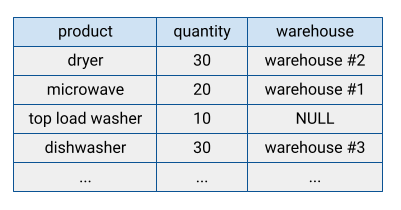
\includegraphics[scale=0.7]{obrazky-figures/row-oriented-store.png}
 \caption{\centering Príklad uskladnenia dát v riadkovo orientovanej databáze. Prechádzať dáta po riadkoch predstavuje musieť prehľadať všetky jeho stĺpce.}
 \label{img:row-oriented-store}
\end{center}
\end{figure}


Riešenie, ktorým BigQuery tento problém adresuje je použitie orientácie na jednotlivé stĺpce. 
Ukladaním dát v stĺpcovom formáte, a teda ukladaním každého stĺpca separátne umožňuje prehľadávať dataset bez viazania sa na všetky ostatné stĺpce.
Tým sa efektívne znižuje množstvo dát, ktoré sa prehľadávajú naraz.
Takto je databáza optimalizovaná pre analýzy nad obrovským množstvom uložených záznamov \cite{google-bq}.

\begin{figure}[htb]
\begin{center}
 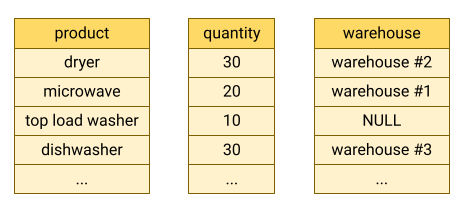
\includegraphics[scale=0.7]{obrazky-figures/column-oriented-store.png}
 \caption{\centering Príklad uskladnenia dát s využitím orientácie na jednotlivé stĺpce. Dáta je takto možné prehľadávať rýchlejšie a efektívnejšie, pričom sa spracuje menší objem dát. To vyhovuje používateľom BigQuery, ktorí sú obmedzení dostupným objemom dát \mbox{(viď platobné plány BigQuery na konci tejto sekcie).}}
 \label{img:column-oriented-store}
\end{center}
\end{figure}

Dáta skladované v BigQuery sú organizované do skupín klasických databázových tabuliek nazývaných \textbf{dataset}.
Na GCP je dostupné množstvo datasetov pre prehľadávanie.
Je nutné si najprv založiť \textbf{Google Cloud projekt} na oficiálnej stránke, ktorý slúži ako menný priestor pre zdroje, ktoré užívateľ do neho pridáva a používa.
K dátam je možné priamo pristupovať prostredníctvom troch rozhraní: \cite{google-cloud} 
\begin{enumerate}
    \item Google Cloud Console

    Webové grafické rozhranie pre spravovanie Google Cloud projektov. 
    Časť Google Cloud Console, ktorú užívatelia môžu využiť špecificky na prehliadanie dát BigQuery sa nazýva \textbf{BigQuery Studio}.
    Výhodou tohto spôsobu pracovania so zdrojmi je vysoká úroveň interaktivity, ktorú ponúka zabudované integrované vývojové prostredie pre prácu s dátami. 
    
    \item BigQuery nástroj príkazového riadku

    Pre zobrazovanie databáz a tabuliek, prehľadávanie a spravovanie dát v prostredí príkazového riadka je možné využiť nástroj s názvom \textbf{\code{bq}}. 
    
    \item BigQuery klientske knižnice

    Vďaka klientským knižniciam implementujúcim komunikačné rozhranie s BigQuery je taktiež dostupná možnosť programovo manipulovať a prehliadať zdroje priradené k užívateľskému projektu.
    Táto možnosť je vhodná pre predom definované, opakované úlohy, ktoré či už požadujú zdroje na vstupe, alebo ich počas svojho behu nahrávajú, prípadne upravujú podľa potreby.
\end{enumerate}

\pagebreak

Pri využití ktorejkoľvek z týchto možností platí, že prehliadanie a manipuláciu dát umožňuje jazyk SQL (Structured Query Language).
Ide o zaužívaný štruktúrovaný jazyk pre správu dát uložených v databáze.
V prostredí BigQuery sa používa dialekt pre SQL nazývaný \textbf{GoogleSQL}\footnote{\href{https://cloud.google.com/bigquery/docs/reference/standard-sql/query-syntax}{https://cloud.google.com/bigquery/docs/reference/standard-sql/query-syntax}} \cite{google-bq}.

Ako už bolo uvedené, HTTP Archive ukladá svoje výstupné dáta práve do Google Cloud.
Tieto dáta sa nachádzajú práve v Google Cloud Console dostupné ako \textbf{zdroj} (anglicky resource), ktorý si môže prihlásený používateľ pridať do svojho projektu.
Po pridaní tohto zdroja s priradeným názvom \code{httparchive} do projektu\footnote{\href{https://github.com/HTTPArchive/httparchive.org/blob/main/docs/gettingstarted\_bigquery.md}{https://github.com/HTTPArchive/httparchive.org/blob/main/docs/gettingstarted\textunderscore bigquery.md}} sa sprístupnia pre používanie nasledovné datasety: \cite{httparchive-repo}

\begin{itemize}
    \item \code{summary\_pages}:

    Obsahuje detaily o jednotlivých web stránkach ako časy ich načítania, počet žiadostí o jej zdroje, typy zdrojov a ich veľkosti.
    Taktiež sú tu informácie týkajúce sa presmerovaní, vzniknutých chýb, použitých služieb ako CDN\footnote{\href{https://www.cloudflare.com/learning/cdn/what-is-a-cdn/}{https://www.cloudflare.com/learning/cdn/what-is-a-cdn/}} a iné.
    
    \item \code{summary\_requests}:

    Nachádzajú sa tu dáta o konkrétnych objektoch načítaných ako už spomínané zdroje pre web stránky v datasete \code{summary\_pages}.
    V dátach je možné prehľadávať ako boli zdroje načítané priamo v hlavičkách HTTP odpovede, v ktorej prišli zo serveru poskytujúceho danú stránku.
    
    \item \code{pages}:

    Extrahované HAR súbory pre každú URL z prehľadávaných web stránok.
    
    \item \code{requests}:

    Extrahované HAR súbory pre každý zdroj jednotlivých prehľadávaných web sránok \mbox{v \code{pages} datasete}.
    
    \item \code{response\_bodies}:

    Extrahované HAR súbory obsahujúce celé telo HTTP odpovede z každej URL prehľadávaných web stránok.
    Ide o veľmi veľké tabuľky, ktoré môžu dosahovať veľkosť \mbox{v jednotkách terabajtov (TB)}.
\end{itemize}

BigQuery zdroj \code{httparchive} sprístupňuje aj niekoľko ďalších datasetov, no práve tie spomenuté vyššie tvoria sadu dôležitých, ktorými sa táto práca zaoberá. 

Každý z týchto datasetov obsahuje tabuľky nazvané podľa rovnakej konvencie --- dátum vykonaného zberu dát a prostredie, v akom prebiehal.
Dátum je definovaný formátom YYYY\_MM\_DD, kde YYYY predstavuje rok, MM mesiac a DD deň. Prostredie môže byť buď počítačové alebo mobilné, ako sa spomína už v sekcii \ref{fetching-data}.
Príkladom názvu tabuľky teda môže byť '\code{2023\_01\_01\_mobile}' alebo '\code{2023\_01\_01\_desktop}'.

\pagebreak

\begin{figure}[htb]
\begin{center}
 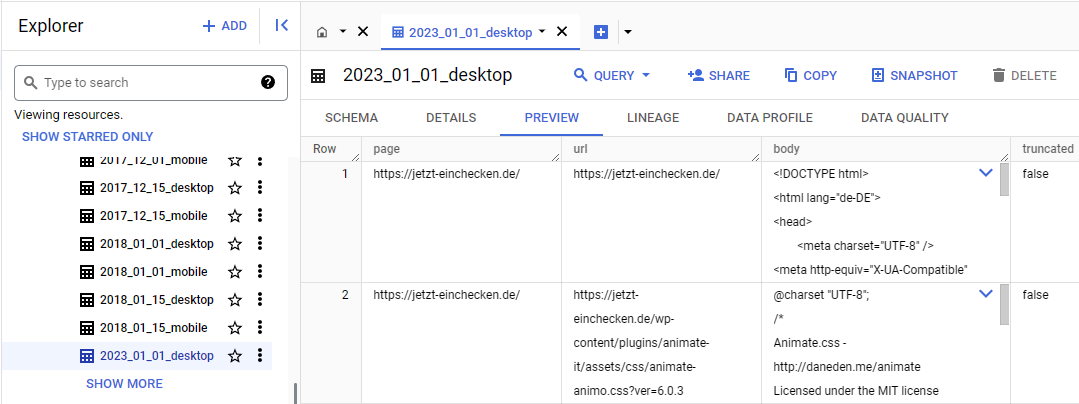
\includegraphics[scale=0.53]{obrazky-figures/bigquery_response_bodies.png}    
 \caption{\centering Otvorené okno v GCP BigQuery pri pohľade na otvorený prehľad datasetu '\code{2023\_01\_01\_mobile}'. 
 Jednotlivé uložené položky sú: \code{page}, \code{url}, \code{body} a \code{truncated}.}
 \label{img:bigquery-example-table}
\end{center}
\end{figure}


Za použitia GoogleSQL je možné datasety kombinovať a vytvárať komplexné sady dát (ako na obrázku \ref{img:bigquery-example-query}) pre ďalšiu analýzu.
Prehľadávaním týchto dát a sledovaním HTTP hlavičiek je možné dopracovať sa k HTTP odpovediam, ktoré obsahujú hlavičky (pravidlá) technológie NEL.
Každú doménu, ktorá vo svojich odpovediach zaslala hlavičku NEL, môžem skúmať ako doménu s nasadeným monitorovaním NEL.

\begin{figure}[!htb]
\begin{center}
% height=8.401cm
 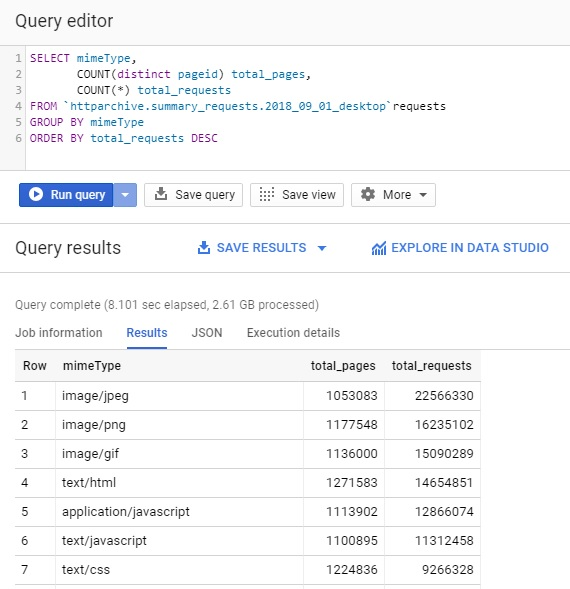
\includegraphics[width=11cm, height=10.0125cm]{obrazky-figures/mimeType_summary_example_query.jpg}    
 \caption{\centering Ukážka vytvorenia vlastnej sady dát v prostredí GCP BigQuery. Za použitia príkazov GoogleSQL sú dáta transformované na zoznam typov MIME podľa ich využitia na stránkach uvedených v dátach.}
 \label{img:bigquery-example-query}
\end{center}
\end{figure}

\pagebreak

Čo sa platieb týka, GCP BigQuery pre užívateľov poskytuje bezplatný plán s nastavenými limitmi pre využívanie konkrétnych funkcií.
\textbf{Bezplatný plán} zahŕňa 1TB procesnej kapacity dát a 10GB úložného priestoru pre vlastné dáta, pričom dochádza každý mesiac \mbox{k obnove týchto bezplatných zdrojov}.
Po prečerpaní kapacity uvedenej v tomto pláne je nutné akékoľvek ďalšie operácie doplatiť.
Zoznam spôsobov, akými je možné zaplatiť za navýšenie spomenutých kapacít je rozsiahly, no pre prípady použitia tejto práce je relevantný platobný plán zvaný On-demand.
\textbf{On-demand plán}, alebo platba podľa potreby sa vzťahuje na procesnú kapacitu, ktorá sa vyčerpáva vykonávaním operácií nad dátami.
Cena za 1TB kapacity je v čase písania práce \$6.25, pričom stále platí, že prvý terabajt je každý mesiac zadarmo \cite{google-bq-pricing}.

\subsection{Pravidelné správy o stave webu}

Okrem samotných dát a prostredia na ich prehľadávanie zostavuje HTTP Archive projekt aj prehľady stavu webu formou interaktívnych grafov reprezentujúcich konkrétnu metriku v oblasti záujmu HTTP Archive.

\subsubsection{Elementárne reporty metrík}
Medzi takéto prehľady patrí napríklad report o zmene priemernej celkovej veľkosti konkrétnej načítanej stránky v kilobajtoch, alebo, taktiež relevantný je aj report zobrazujúci dosiahnuteľnosť HTTP Archive -- počet jedinečných URL analyzovaných týmto projektom (viď obrázok \ref{img:total-urls-report}).

\begin{figure}[!htb]
\begin{center}
 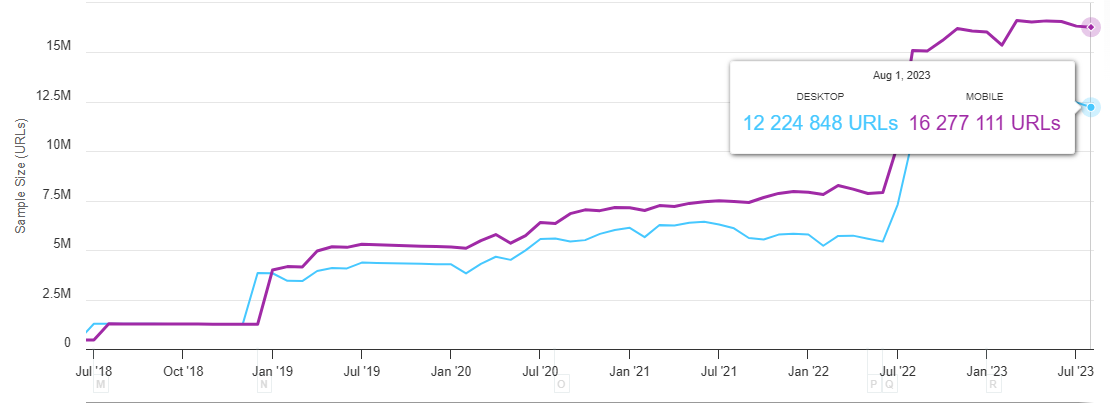
\includegraphics[scale=0.51815]{obrazky-figures/total_urls_report.png}    
 \caption{\centering Report zobrazujúci počet URL adries analyzovaných v rámci projektu HTTP Archive. Graf reportu znázorňuje dáta od dátumu prvého web crawlingu vykonaného v rámci projektu. Momentálny počet URL adries zakomponovaných do datasetov v BigQuery je 12 224 848 pre testy vykonávané na počítači a 16 277 111 pre testy vykonávané zo simulovaného mobilného prostredia.}
 \label{img:total-urls-report}
\end{center}
\end{figure}

\pagebreak

\subsubsection{Web Almanac}
\label{web-almanac}
Na takýchto a mnoho ďalších nízko úrovňových reportoch každoročne stavia aj komplexný report s názvom \textbf{Web Almanac}, ktorý tiež patrí pod túto iniciatívu.
Web Almanac spája elementárne dáta do kontextualizovaných náhľadov, ktoré približujú jeho čitateľom stav webu na vysokej úrovni \cite{httparchive-methodology}.
Posledný report bol už štvrtým vydaním v poradí.
Vďaka skúsenostiam z predošlých troch rokov autori navýšili relevantnosti metrík, ktoré zahŕňa. 
Všetky tieto skúmané metriky sú zároveň dostupné na GitHub stránkach projektu, kde každú jednu reprezentuje hotový SQL skript spustiteľný priamo v prostredí GCP Big Query.

Celý obsah reportu je dostupný na jeho oficiálnej stránke\footnote{\href{https://almanac.httparchive.org/en/2022/table-of-contents}{https://almanac.httparchive.org/en/2022/table-of-contents}}. 
Každý aspekt jeho prieskumu je zatriedený do svojej vlastnej kategórie, ktorá sa v rámci obsahu označuje ako samostatná kapitola.
Čitatelia tu môžu nájsť napríklad kapitolu zameranú špecificky na JavaScript, použitie WebAssembly na webe, ale aj pre túto prácu relevantnejšie oblasti ako HTTP a bezpečnosť.

Celkovo sa snahou viacej ako 100 prispievateľov podarilo takouto formou štruktúrovane zaznamenať stav webu textovo, ale aj pomocou detailných grafových vizualizácií.
Autori sa snažia zvýšiť rozsah projektu a tým aj počet sledovaných relevantných oblastí tak, že každý rok povzbudzujú nových potencionálnych prispievateľov do pripojenia sa k ich iniciatíve. 

Do budúcna sa bude kvalita Web Almanac reportov zlepšovať. 
V tohtoročnom reporte bude oproti tomu minuloročnému zahrnutých viac ako dvojnásobok vzoriek URL, 
ktoré HTTP Archive podrobí svojmu web crawlingu.
V ideálnom prípade to znamená, že sa dosah podkladov pre report efektívne zdvojnásobí a tým pádom má potenciál byť presnejší a globálne reprezentatívnejší.

Využitie práve tohto reportu by bolo ideálnym spôsobom, ako \textbf{dostať technológiu NEL a jej využitie do verejného povedomia}. 
Spoluprácou s autormi Web Almanac by sa jedna z nových kapitol budúcich vydaní mohla zaoberať technológiou NEL.

% \section{Alternatívy}
% \label{httparchive-alternatives}

% Aj keď je HTTP Archive najvhodnejším zdrojom dát pre účely tejto práce, existujú aj iné, ktoré stoja za zmienku.
% Dáta, ku ktorým máme prístup vďaka tomuto primárnemu zdroju síce sú postačujúce pre rôzne typy analýz. Sú ale dostupné aj zdroje disponujúce špecifickými výhodami, ktoré
% zase umožňujú či už spätne kontrolovať správnosť dát HTTP Archive, alebo na ne nadviazať.
% Z toho dôvodu sú niektoré alternatívy popísané v tejto kapitole.

% \subsection{crawler.ninja}

% Projekt \textbf{crawler.ninja} založený autorom Scottom Helme slúži ako podklad pre jeho prieskum
% webu, v ktorom pozoruje stav bezpečnosti na internete. 
% Výsledky tohto prieskumu autor prvýkrát zverejnil už v roku 2015, no o vytvorení projektu crawler.ninja na svojom blogu píše až v júli 2018 \cite{crawler-ninja}. 

% % \pagebreak

% Úmyslom autora pozorovať bezpečnosť vyúsťuje do jeho periodických reportov týkajúcich sa tejto tématiky. 
% Samotný projekt sa stará o zber dát pre zhotovenie týchto reportov.
% Aj keď zbieranie dát pretrváva do súčasnosti, posledný report od autora bol publikovaný dávnejšie --- 09.12.2021, od kedy zanechal svoju pravidelnosť (aspoň jeden report za rok).

% Crawler.ninja slúži na prehľadávanie webu technikou Web Crawling za cieľom získať dáta o web stránkach, ktoré autor plánuje skúmať.
% Ako vstup do tohto procesu, a teda zoznam použitých URL, sa používa rebríček populárnych stránok Alexa Top 1 milion.

% Crawl sa spúšťa každý deň a získané dáta ukladá (podľa toho čo autor zmieňuje na svojom blogu) do databázy MySQL, z ktorej je následne vytvorený takzvaný databázový export.
% Databázový export predstavuje súbor SQL príkazov, spustením ktorých môže ktokoľvek replikovať pôvodnú databázu aj s obsahom jej tabuliek. 
% Možnosť vytvoriť takýto súbor poskytuje priamo MySQL databáza. 
% Jednou z možností ako ho vytvoriť je použitím pomocného programu na tvorbu databázových záloh --- \code{mysqldump} \cite{mysql-doc}.
% Toto je dôležité pre toho, kto chce výsledné dáta použiť. 
% Na oficiálnej stránke crawler.ninja autor tieto súbory periodicky (ale nie priebežne za každý deň) zverejňuje pod licenciou \textit{CC BY-SA 4.0}, takže sú všetky získané dáta použiteľné pre študijné, ale aj komerčné účely potencionálnych záujemcov.
% Sú dostupné vo forme priamo stiahnuteľných archívov ZIP, pomenovaných vždy podľa dátumu, za ktorý boli nazbierané.
% Ako je spomenuté vyššie, ten, kto chce dáta na svoje účely využiť si ich musí najskôr importovať do svojej databáze MySQL, kde s nimi môže začať pracovať.
% Docieliť toho je možné napríklad shell príkazom \code{\textbackslash source} v administrátorskej konzole MySQL \cite{mysql-doc}.

% Mimo uvedených dát v podobe databázových exportov sú od Scotta dostpné taktiež konkrétne, pre neho významné, postupne nazbierané metriky, ktoré v reportoch o svojich prieskumoch používa či už priamo, alebo v rôznych kombináciách pri tvorbe grafov. Taktiež sú zverejnené na jeho webe\footnote{\href{https://crawler.ninja/files/}{https://crawler.ninja/files/}}.

% \subsubsection{Výhody a nevýhody}

% Na rozdiel od HTTP Archive je crawler.ninja web crawl spúšťaný každý deň a nie len 
% na začiatku mesiaca. To znamená, že dáta v tomto prípade nadobúdajú vyššiu granularitu. Crawler.ninja taktiež všetky svoje zdroje ponúka bezplatne.
% Avšak, problém tu pôsobí skutončosť, že dáta nie sú zverejňované v reálnom čase, ale manuálne autorom po nejakej dobe od ich získania. Tomu nasvedčuje priamo oficiálna stránka projektu, kde sa často nezobrazujú stiahnuteľné archívy s dátami až po aktuálny dátum.
% Ešte väčší potenciálny problém predstavuje skutočnosť, že sa archívy príliš staré vymazávajú, a teda sú dostupné dáta iba do nedávnej minulosti.
% Obdobie dostupnosti dát, predstavujúce rozdiel dátumov najaktuálnejšieho dostupného archívu a najstaršieho archívu, je v čase písania tejto práce presne 1 rok, 10 mesiacov a 23 dní \cite{crawler-ninja}.


% \subsection{Ešte som niečo našiel ale nestihol pripísať :)}
